\begin{figure}[h!]
    \hspace{-1.5em}
    \begin{subfigure}{0.5\textwidth}
    \centering
    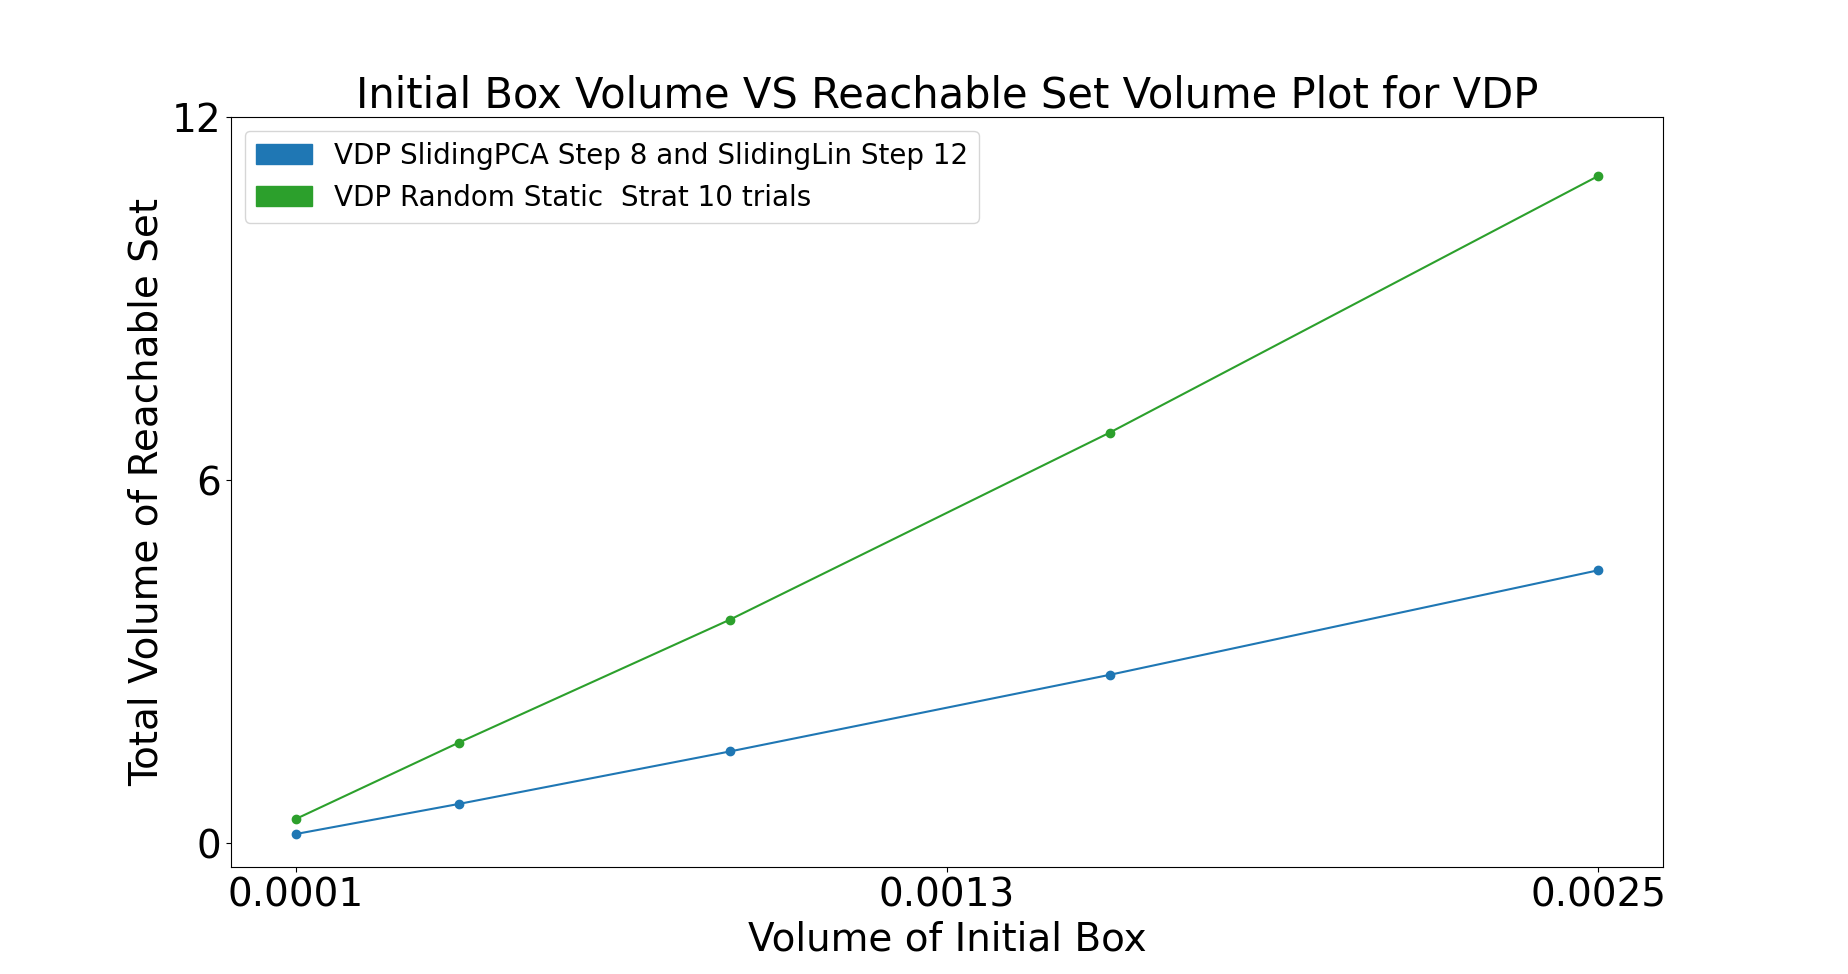
\includegraphics[width=1.1\textwidth, height=0.75\textwidth]{figures/InitVolVSReachVol/VDPInitReachVolRanStrat.png}
    \caption{Vanderpol}
    \end{subfigure}%
    \begin{subfigure}{0.5\textwidth}
    \centering
    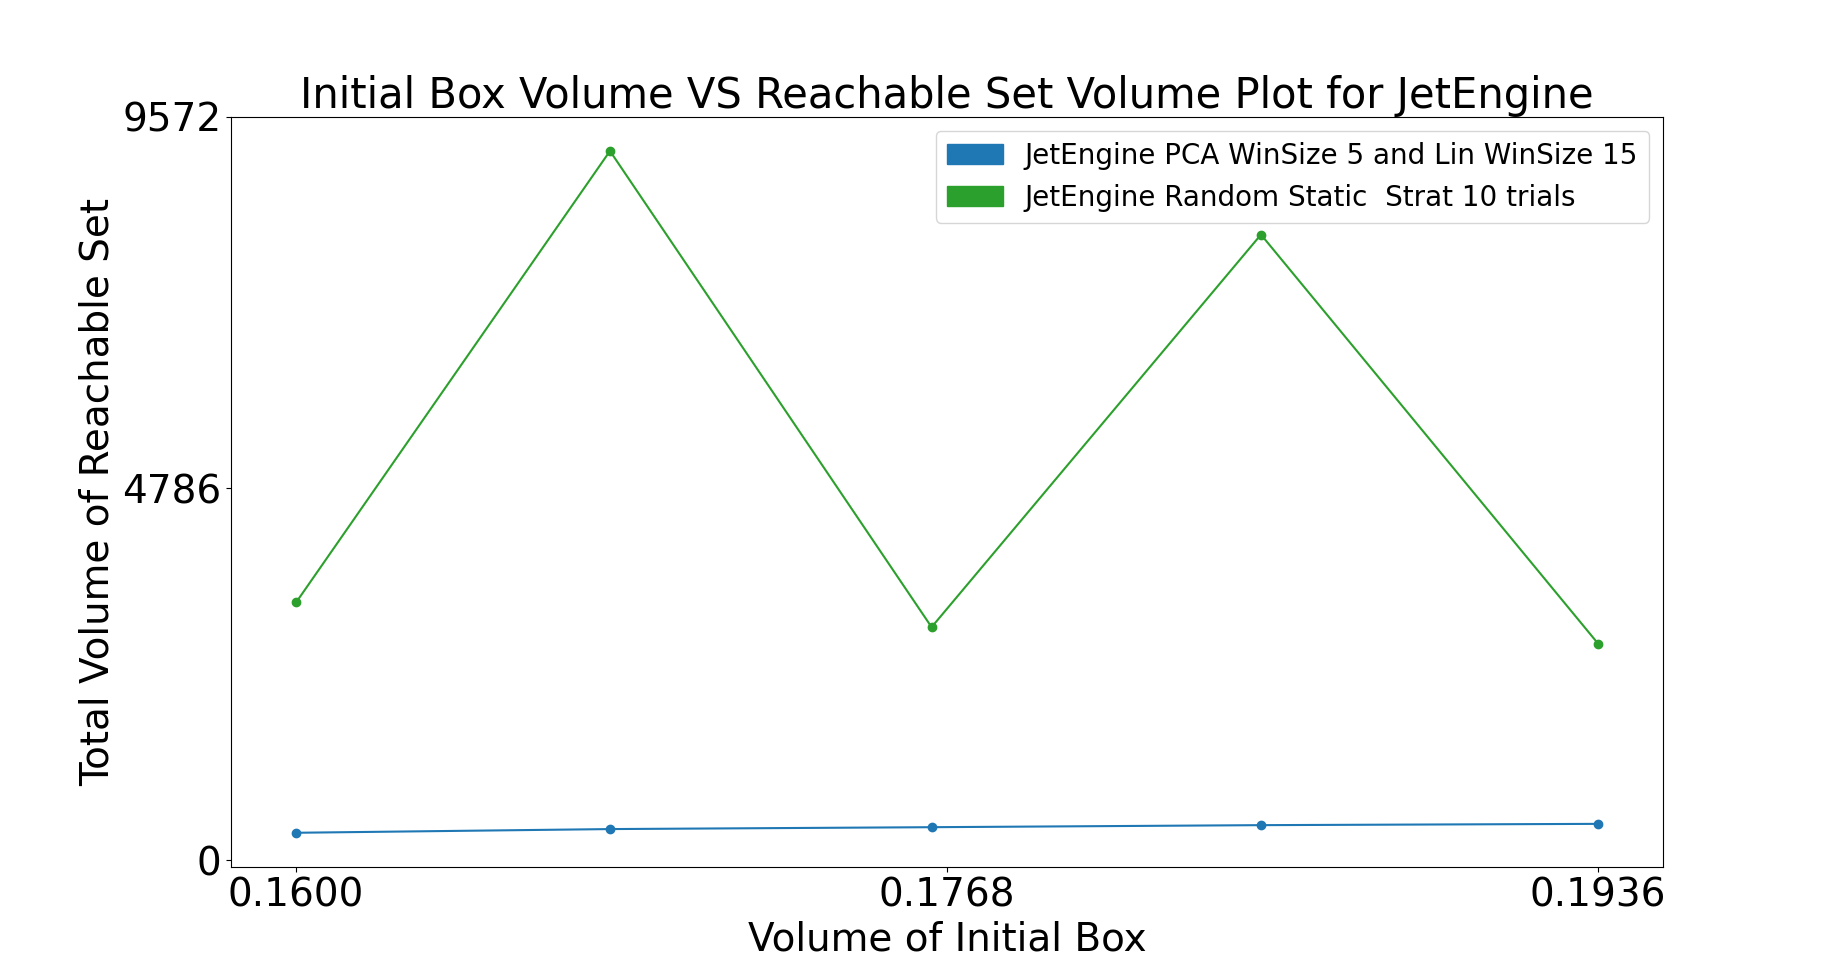
\includegraphics[width=1.1\textwidth, height=0.75\textwidth]{figures/InitVolVSReachVol/JetEngineInitReachVolRanStrat.png}
    \caption{Jet Engine}
    \end{subfigure}

    \hspace{-1.5em}
    \begin{subfigure}{0.5\textwidth}
    \centering
    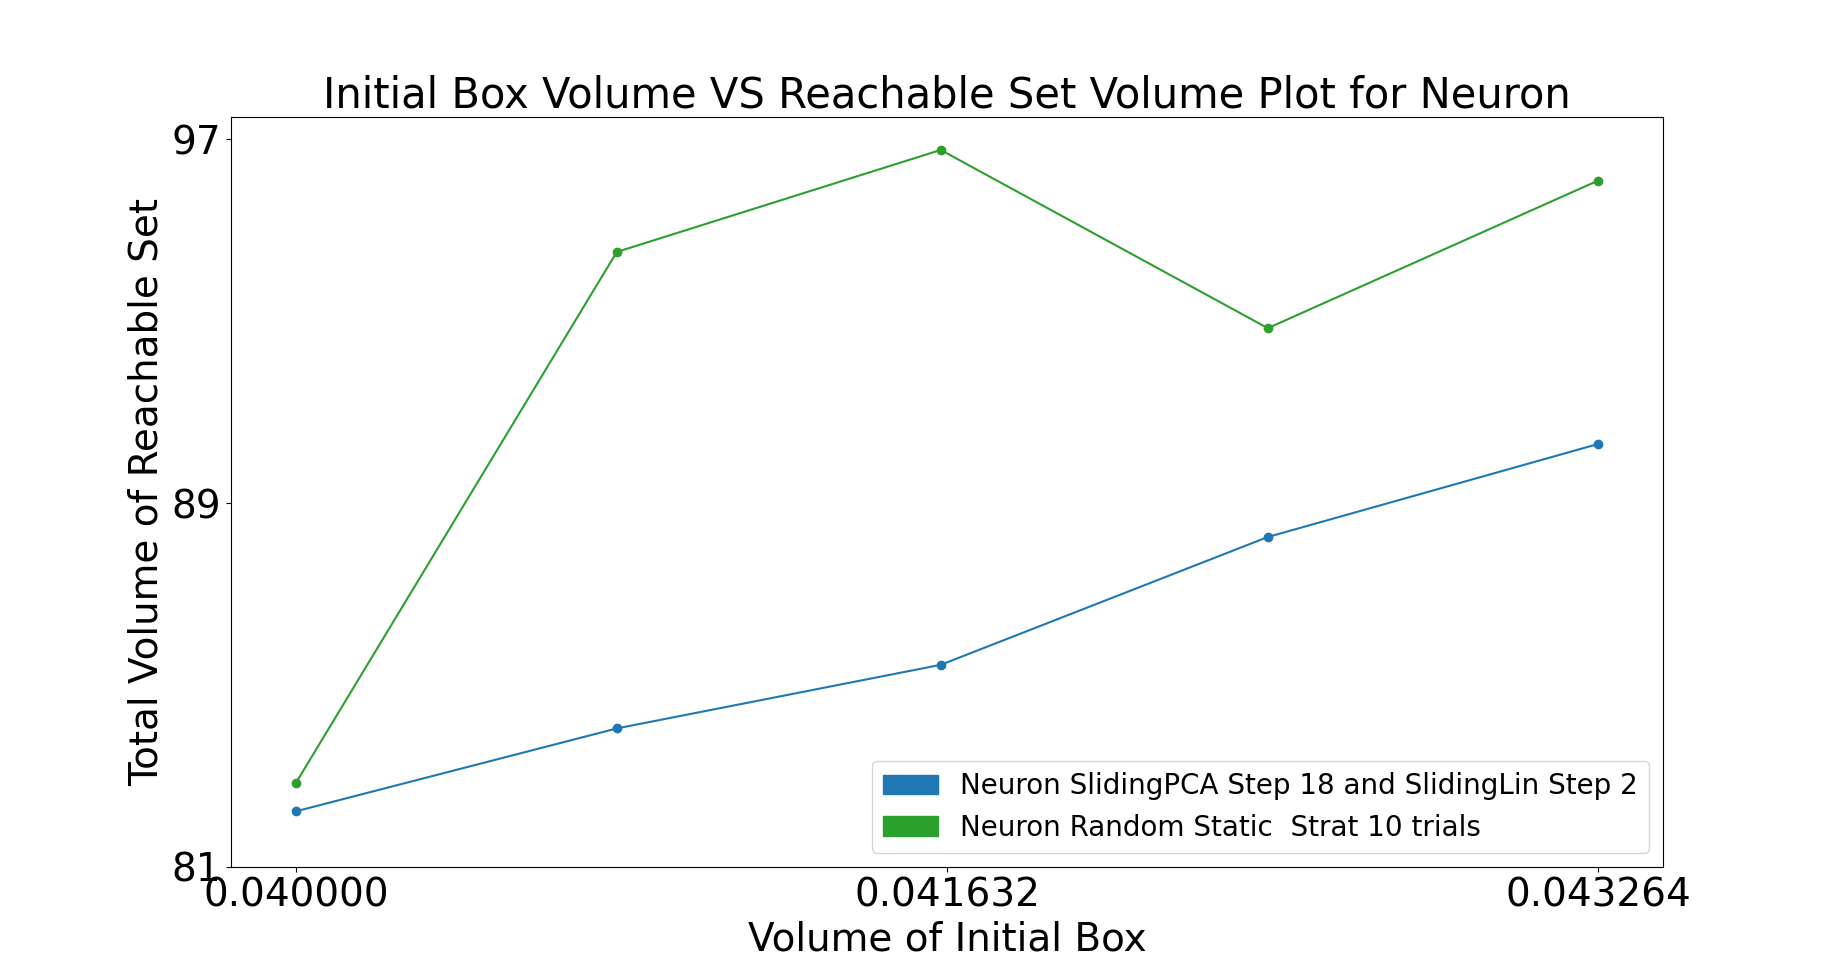
\includegraphics[width=1.1\textwidth, height=0.75\textwidth]{figures/InitVolVSReachVol/NeuronInitReachVolRanStrat.png}
    \caption{Neuron}
    \end{subfigure}%
    \begin{subfigure}{0.5\textwidth}
    \centering
    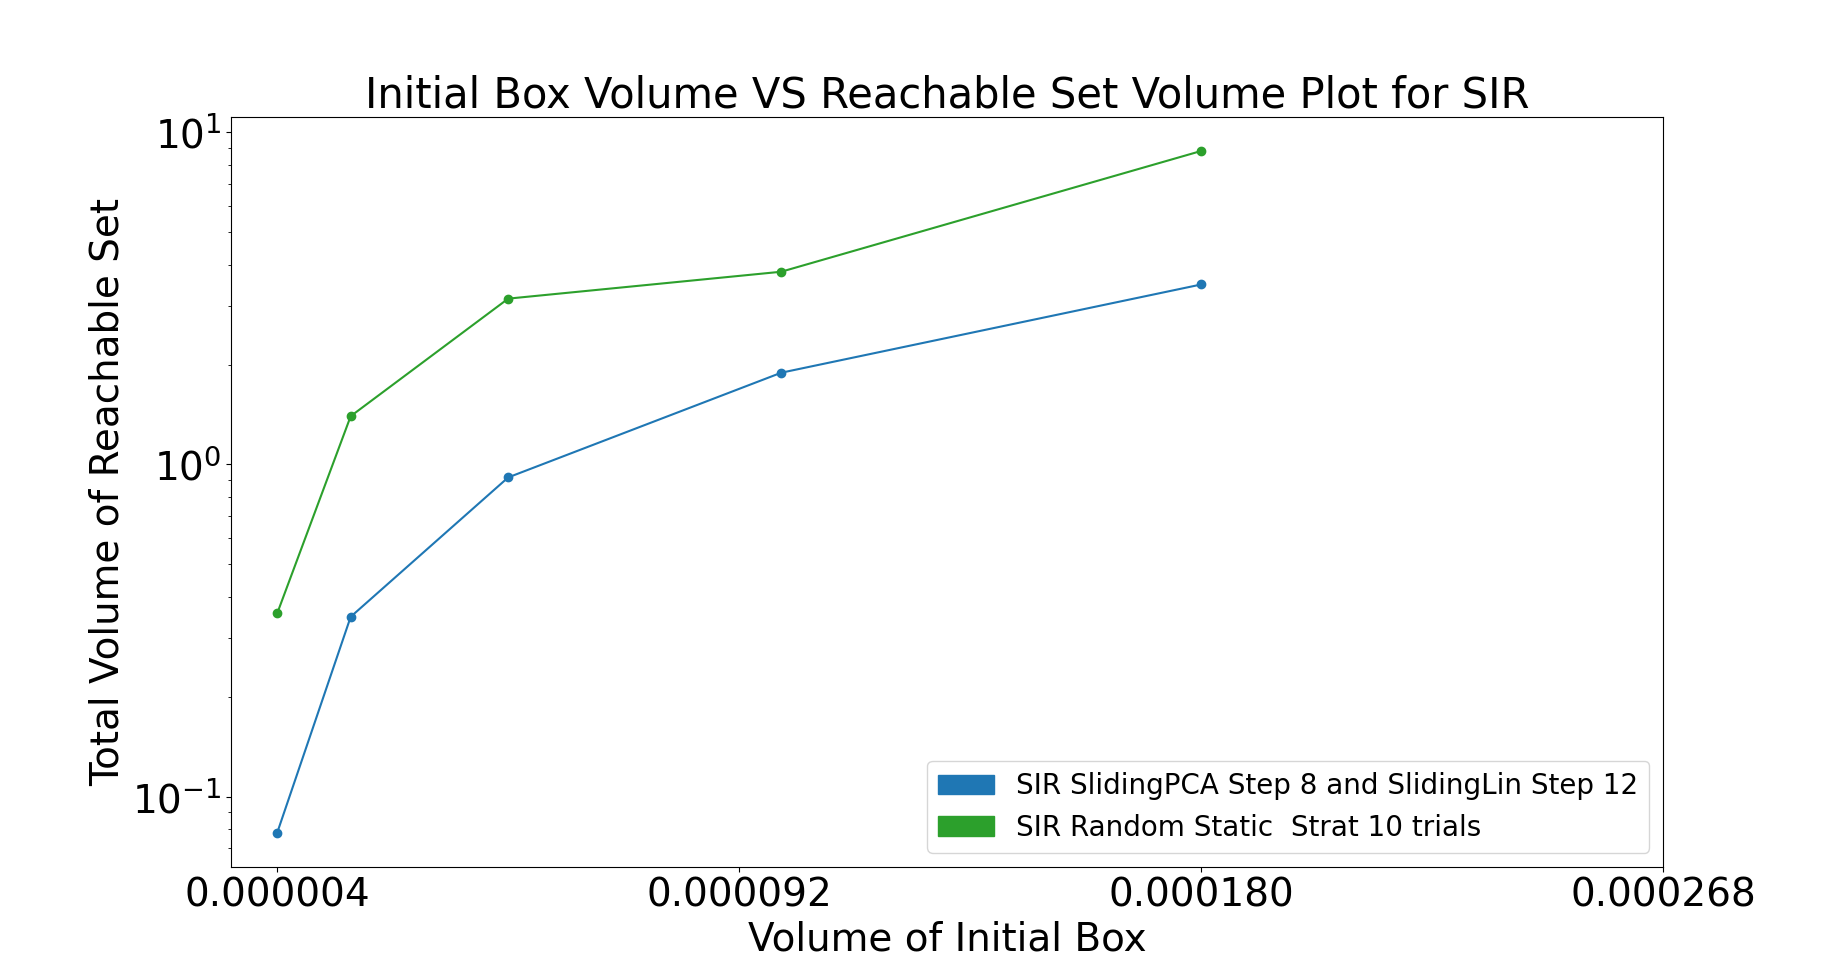
\includegraphics[width=1.1\textwidth, height=0.75\textwidth]{figures/InitVolVSReachVol/SIRInitReachVolRanStrat.png}
    \caption{SIR}
    \end{subfigure}

    \hspace{-1.5em}
    \begin{subfigure}{0.5\textwidth}
    \centering
    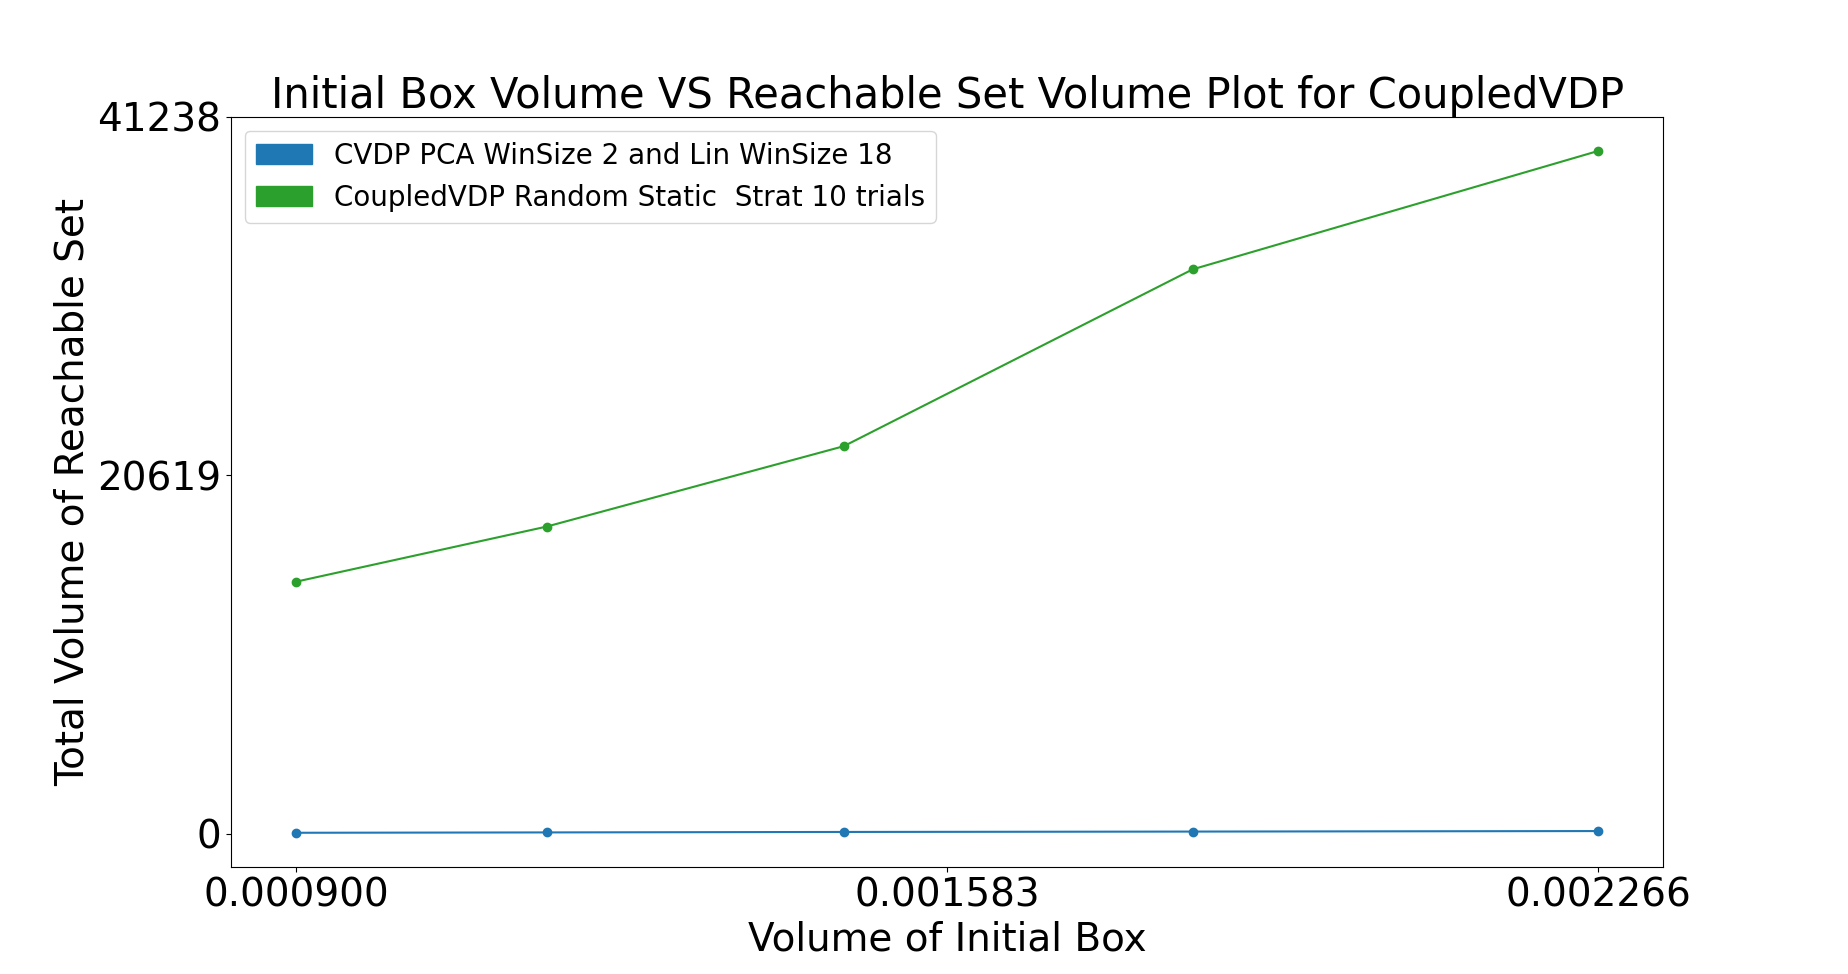
\includegraphics[width=1.1\textwidth, height=0.75\textwidth]{figures/InitVolVSReachVol/CVDPInitReachVolRanStrat.png}
    \caption{Coupled Vanderpol}
    \end{subfigure}%
    \begin{subfigure}{0.5\textwidth}
    \centering
    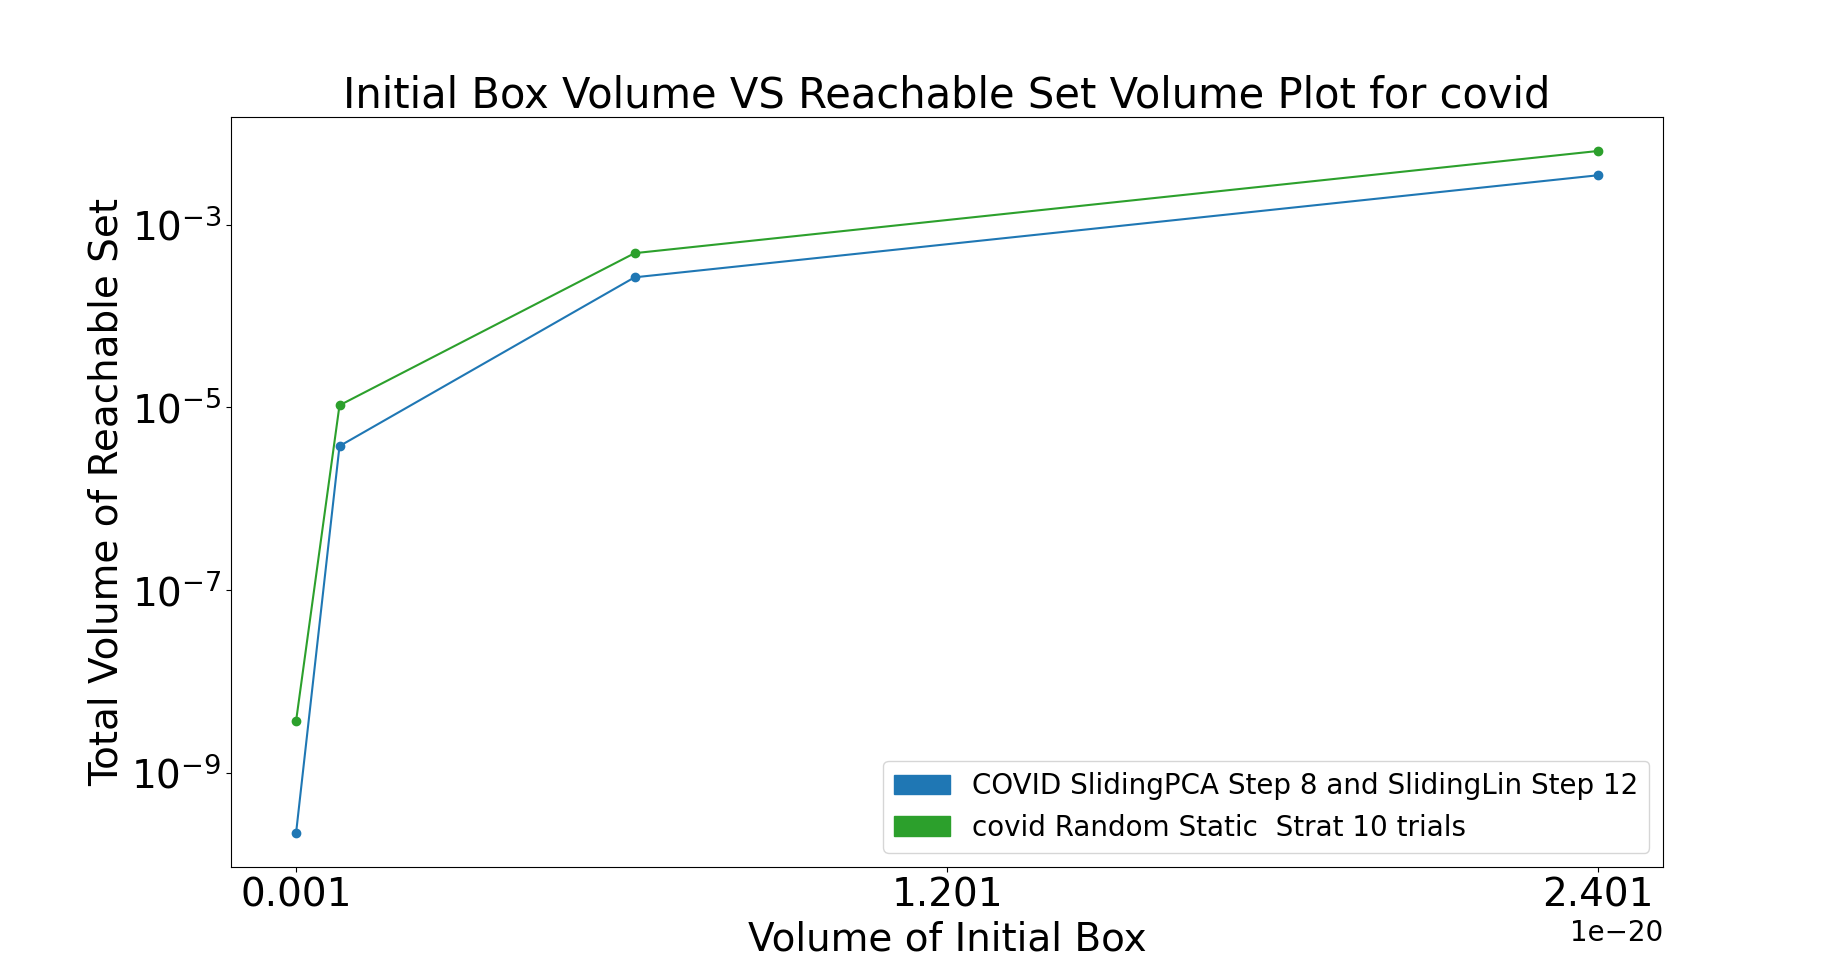
\includegraphics[width=1.1\textwidth, height=0.75\textwidth]{figures/InitVolVSReachVol/CovidInitReachVolRanStrat.png}
    \caption{COVID}
    \end{subfigure}

    \caption{Comparision between random static strategies and the best performing dynamic strategies as the volume of the initial set grows. The total reachable set volumes for random static strategies are averaged over ten trials for each system.}
    \label{fig:RanStaticStratComp}
\end{figure}
